\documentclass[12pt]{article}

\usepackage{amsmath, amsthm, amsfonts, enumitem, graphicx, subcaption, cleveref, tabularx, xpatch, makeidx, setspace, mathptmx, titlesec, fancyhdr, etoolbox, tocloft}
\usepackage[backend=biber,style=numeric]{biblatex}
\usepackage[a4paper,top=3cm,bottom=2.5cm,left=2.5cm,right=2.5cm]{geometry}

\makeindex

\addbibresource{src/bib/references.bib} 

% TIPOGRAPHY
% Page settings
\pagestyle{fancy}
\fancyhf{}
\fancyfoot[C]{\thepage}

% Line spacing
\onehalfspacing

% Paragraph indent
\setlength{\parindent}{0.7cm}

% Chapter and section titles
\titleformat{\chapter}[display]{\bfseries\Huge}{\chaptername\ \thechapter}{20pt}{\bfseries\LARGE}
\titleformat{\section}{\normalfont\Large\itshape}{\thesection}{1em}{}

% Blockquote setup
\newenvironment{blockquote}{\begin{quote}\onehalfspacing\fontsize{11}{13.2}\selectfont}{\end{quote}}

% Footnotes
\renewcommand{\footnotesize}{\fontsize{10}{12}\selectfont}
\setlength{\footnotesep}{\baselineskip}
\appto\footnotesize{\singlespacing}


% CUSTOM COMMANDS
\newcommand{\meqref}[1]{Eq.\ref{#1}}
\newcommand{\mfigref}[1]{Fig.\ref{#1}}
\newcommand{\mtabref}[1]{Tab.\ref{#1}}
\newcommand{\mappendixref}[1]{Appendix \ref{#1}}
\newcommand{\indfunc}[1]{\textit{\textbf{1}}_{#1}}
\makeatletter
\xpatchbibmacro{textcite}{%
  \printnames{labelname}%
}{%
  \printfield[citetitle]{labelname}%
}{}{}
\DeclareCiteCommand{\fancycite}
  {\usebibmacro{prenote}}
  {\textit{\printnames{labelname}%
   \ifnum\value{citecount}=1 \printtext{ et al.} \fi%
   \printfield{year} \textsuperscript{\printfield{labelnumber}}}}
  {\multicitedelim}
  {\usebibmacro{postnote}}
\makeatother
\makeatletter
%\DeclareFieldFormat{labelnumber}{\textit{\mkbibsuperscript{#1}}}
\DeclareCiteCommand{\ucite}
  {\usebibmacro{prenote}}
  {\textsuperscript{\textit{\printfield{labelnumber}}}}
  {\multicitedelim}
  {\usebibmacro{postnote}}
\makeatother

% Document starts here
\begin{document}

\title{Properties and Implementation of Sequential Expansion of Latin Hypercube Sampling for Simulation Design}
\author{Crespi Alessandro, Gerosa Davide, Boschini Matteo}
\date{July, 2024}
\maketitle

% \begin{abstract}
% \end{abstract}

\section{Introduction}
Simulation design is a branch of Statistics that studies ways to build better simulations, intended as tools for enhancing the comprehension of phenomena, which have become widely used in mathematics, physics, economics, mechanics, and every scientific field as experimental tools for proofing theories, interpolating real sampled values, and, more generally, generating predictive models that try to explore uncharted traits, features, and peculiarities, perhaps intuitively or roundly developed in the early stages of the study of a specific problem.

Since the advent of hybrid mechanical-electrical programmable calculators such as IBM's machines, the first of their kind to be really useful in engineering, scientists have them involved in heavy computations for experiments. Following, in 1969, the Kennar and Stone's Computer Aided Design for Experiments (CADEX)\ucite{kennard1969} proposal for computer-driven experiments has led to spread up a broad variety of Computer-based simulation methods.

Eventually, computer-based simulations are a set of strategies that benefit from mathematical modelling techniques based on discrete known points placed in a limited parameter space, hereafter samples, and the computer programmability advantage has been used to design, shape and enhance a specific subset of samples that satisfy the desired properties, hereafter sample sets. 

The general concept of computer simulation has been defined in the past few decades, it's based on the following key ideas: taking into account a desired behavior $ F $ the experimenters have an interest in, F has to be explored through its $ N $ real parameter space; the algorithm takes randomly samples from a standard $ N $-dimensional hyperspace $ \Omega $ and arranges the sample set for the simulation; afterwards, the simulation is carried out by evaluating $ F $ over the sample set and eventually producing a so-called surrogate model. The class of algorithms meant to implement this abstraction is commonly named as Sampling Methods.

A critical consideration when evaluating sampling methods is the trade-off between exploration and exploitation. An exploration-oriented sample set maximizes the simulation skill of seeking key features over the studied behavior. Exploration has been depicted as a model-free practice, so that it does not base its own actions on the model (behavior) evolution or any other on-site response. On the other hand, exploitation is an auxiliary mechanism that aims to better assist the simulation by deploying samples in strategic placements that prevent exploration from exceeding the prediction surrogate made upon a key region (such as overshooting an optima or mismatching a discontinuity for a steep slope).

The most iconic sample method for simulations is obviously the pseudo-random sampling, lightened of every other criteria, namely the Monte Carlo Sampling or MCS (\fancycite{metropolis1987})  which it has been proposed as fundamental design of sampling methods. Quasi-Monte Carlo methods are a class of sampling algorithms based on Monte Carlo, indeed, but without a proper random drawing of sample points from the parameter space, instead, points are sequentially extracted in order to satisfy one or multiples criteria as best as the computational time required remains acceptable.
 
Many criteria have been theorized and tested; each of them has its own best scenario, which it'd be better to apply to. An updated, summarized list of the most remarkable ones is shown and commented in section \cref{sec:lhs_properties} in \cref{tab:remarkable_criterions}. As per the interest of this paper, the reader is going to learn about the space-filling class of criteria and the one-projection property (also known as non-collapsing property or projective property); the latter has been widely known because of the Latin Hypercube Sampling (LHS), topic of this research and explained afterwards. The space-filling design of points measures the quality of a sample set to be spread evenly across an hyperspace; the way space-filling is defined determines the final aspect of the sampling. On the other hand, a sample set, in $P$-dimensional space, admits the one-projection property if and only if each projection of every sample $x$ on a specific axis does not overlap onto each other's interval $I_j$. These $I_j$ intervals are well-known fixed-width slices of the limited volume of parameter space taken into examination (e.g., a volume $[0,1)^N$ ) and the number of intervals is equal to the number of samples taken. So, the non-collapsing property prevents samples to fall into a busy "private space" (which has been occupied by another sample). Furthermore, given that the number of intervals and the size of the sample set is equal, it does ensure there are no empty intervals across the parameter space.

The authors used to work with sampling methods for simulation design, more likely LHS designs, in Astrophysics related experiments, such as simulating black hole binary systems collapsing, which obviously requires a massive amount of computational time and many different parameters. The authors often experienced difficulties predicting how long it would take to run a full simulation given $N$ known sampling points in a $P$-dimensional space. This situation forces them to reserve more machine time on a shared company supercomputer for experiments than they really need. In order to better spend the reserved machine time left after the execution of the first run of sampling points, the authors designed an algorithm that adds up points to the previous LHS' sample set and another set of samples that has been drawn by the expansion algorithm in order to preserve the non-collapsing property of both sample sets together.

The authors of this paper propose a algorithm called "Expansion of an LHS" that, indeed, takes a already existing Latin Hypercube Sampling' sample set and propose a new set of points samples in the same parameter hyperspace which are suppose to maximize the non-collapsing property of the samples altogether. 
The original sample set is referred as "starting set" and the add-on samples as "expansion set". The whole sample set joined together by both is called "expanded simulation".

The paper is structured as follows: 1. Latin Hypercube Sampling [...]; 2. Expansion algorithm [...]; 3. .....; X. Conclusion .

\section{LATIN HYPERCUBE SAMPLING}
\subsection{What is an LHS? }
According to the Handbook of Computational Designs (2nd edition, 2006) \ucite{colbourn2006}, the first appearance in history of the "Latin Square" has to be attributed to the Korean mathematician Choi Seok-jeong, who described it, using modern terminologies, as a $N \times N$ matrix (the square) with $N$ distinct symbols, appearing $N$ times each but precisely once per type for each row and column. The suffix "Latin" has been inspired by the efforts that Leonhard Euler has put into this topic while defining a general theory for Latin Squares \ucite{wiki_latin_square} and using Latin letters as symbols to fill the square up with. See Fig.1 for an example with 4 objects.

\begin{figure}[h]
    \centering
    \begin{subfigure}[b]{0.45\textwidth}
        \centering
        \vtop{
        	\vspace{0pt}
        	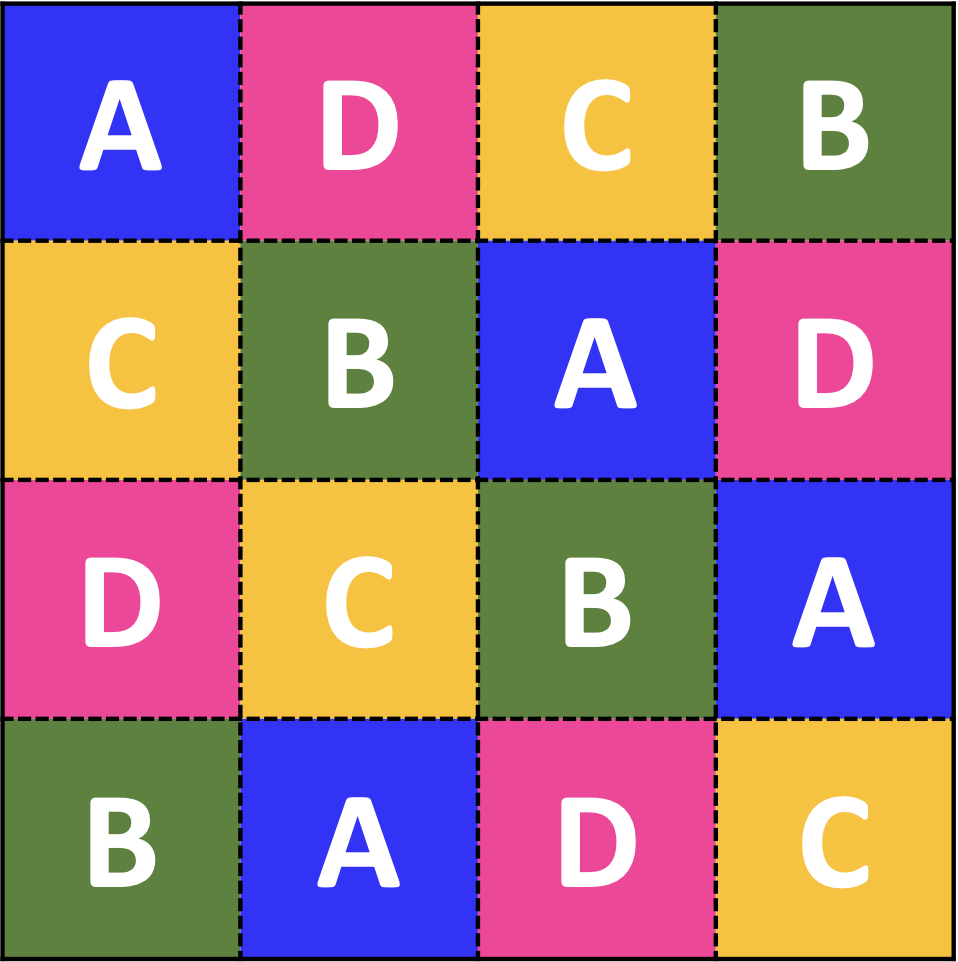
\includegraphics[width=\textwidth]{src/imgs/latin_square_letters_and_colours.png}
        	\caption{A Latin 4x4 Square with 4 distinct symbols, both letters or colors either, arranged so that no letter occurs more than once in a row or a column}
        	\label{fig:latin_square_a}
        }
    \end{subfigure}
    \hspace{0.05\textwidth}
    \begin{subfigure}[b]{0.45\textwidth}
        \centering
        \vtop{
        	\vspace{0pt}
        	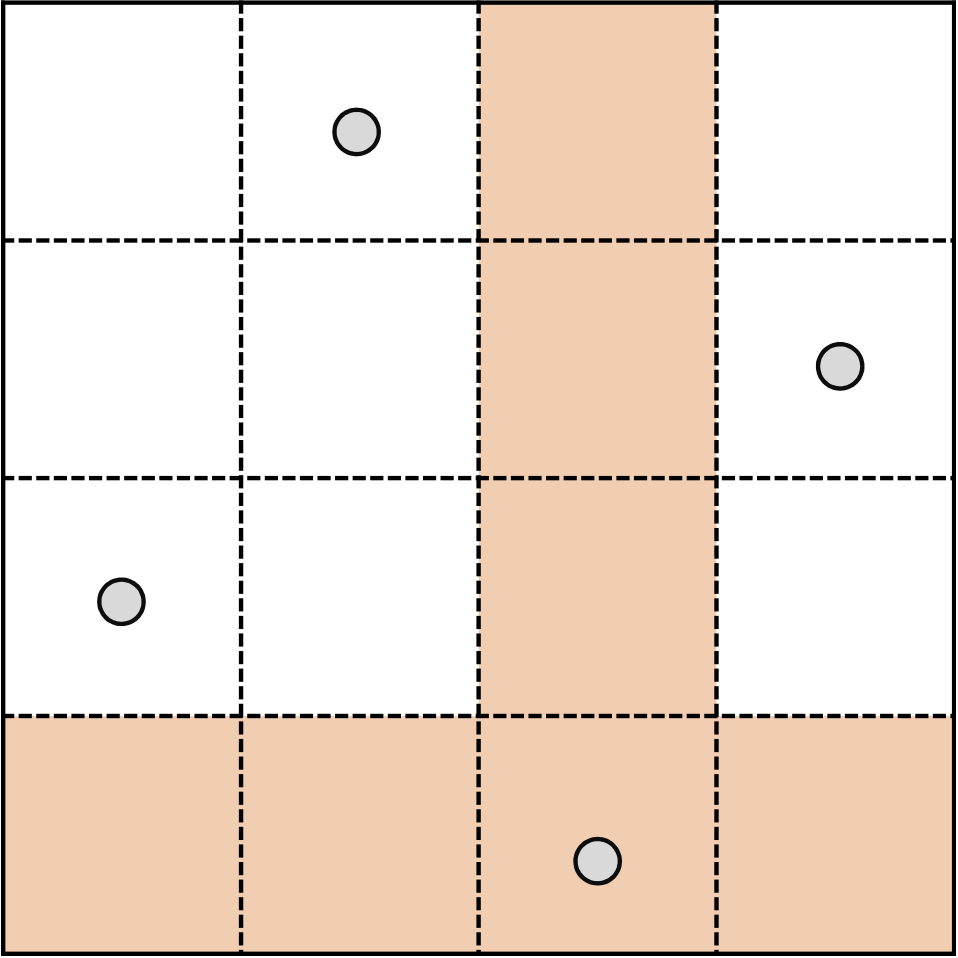
\includegraphics[width=\textwidth]{src/imgs/latin_square_skeleton.png}
        	\caption{The skeleton of (a) Latin Square highlighting only the D (or PINK) symbol positions, it's easily noticeable how the positions does not overlap onto each other's row and column both}
        	\label{fig:latin_square_b}
        }
    \end{subfigure}
    \caption{The images were kindly taken [inserting sheikholeslami2017 throws an error?]
    %\fancycite{sheikholeslami2017}. throws error
    }
    \label{fig:latin_square}
\end{figure}

Per the interest of this paper, which doesn't aim to study how the symbols behave with each other and several algebraic combinatorics considerations, and for sake of clarity, the $N$ number of distinct symbols factor is not taken into account anymore. Instead, it has been considered a sole symbol, hereafter "sample", which has to obey the "do not cross into each other's row and column", hereafter non-collapsing property. The sample must occur in the hyper-matrix exactly $N$ times.

Generally, we can speak of "Hypercubes" by transposing the classic 2-dimensional matrix concept (depicted as a grid in Fig.1a) into a more complex multidimensional matrix where $N$ samples are placed such that each one lies exactly once on each fiber (in literature, a "fiber" of a multidimensional matrix is the general term for a one-dimensional substructure in any dimension (mode) of a tensor. e.g. In a 2D matrix, the fibers of the first and second dimensions are respectively "rows" and "columns").

The modern approach of LHS is not supposed to place symbols in matrices but, instead, attempts to place $N$ samples on hyperspaces that represent the examined parameter space of the interested model, where each axis is associated with a different parameter. The parameter hyperspace has a limited span, which is the hyper-volume $[0,1)^P$, commonly used in literature, which represents, again, a hypercube. However, some texts use a different standard, and they let the parameter space take place in a $[-1,1)^P$ hypercube. Every parameter axis is sliced into smaller consecutive intervals of width $\frac{1}{N}$ that consequently depict the sub-region where each coordinate of the points is sampled randomly. In anticipation for further definitions, we provide a indexing system for intervals; in any dimension of the hypercube with $N$ intervals, for each $j$ from 0 to $N-1$, the j-th interval's boundaries are:
\begin{equation}
\label{eq:interval_index}
I_j = [\frac{j}{N}, \frac{j + 1}{N})
\end{equation}
With no loss of generality, the examples and considerations designed by the authors of this paper assess the random distribution to be uniform in all intervals. The uniformly distributed samples can be transformed by associated transformation functions for any other distribution (e.g., a Gaussian distribution).

\subsection{How to build a Latin Hypercube Sample Set}
In this section it has been marked out mathematically the construction of an LHS sample. This description is widely used for introducing the topic on many textbooks and lectures and it takes inspiration from the work of X.Kong at al. \ucite{kong}.
Let $S = \{S_1, S_2, ..., S_N\}$ be the Latin Hypercube sample set with $N$ number of samples, where for each $S_i$ its cardinality is $P$ number of dimensions. It is comfortable to use the matrix representation $S_{ij}$ whereof rows are the i-th sample and columns, instead, represents the projection of every sample on each j-th dimension. Then, we introduce the sorted index matrix $A = \{A_{ij} = j - 1\}$ as a tool for trace the intervals index (starting from zero), its purpose will be clearer soon. \\
Given an $A$ index matrix, the preliminary design matrix S is given by: 

\begin{equation}
\label{eq:Sij_def}
S_{ij} = \frac{a_{ij} + u_{ij}}{N}
\end{equation}

where $u_{ij}$ is a uniform distributed variable U[0,1). This preliminary design has the peculiarity to have the samples always placed on the diagonal of the hypercube $[0,1)^P$. Now the index matrix come into use, typically shuffling the original $A$ we attain $B = \{b_{ij}\}$ random permutation, which plugging it  into \cref{eq:Sij_def} describe the uniform random variable $S_{ij}$ living inside the statistical bin identified by the interval index $b_{ij}$. We explicitly write down the uniform random variable $S_{ij}$ involving \cref{eq:interval_index} boundaries for the ij-th interval as well: 
\begin{equation}
\label{eq:rand_variable_Sij}
S_{ij} \text{ $\sim$ } U[\frac{b_{ij}}{N}, \frac{b_{ij} + 1}{N})
\end{equation}

\subsection{Grade of a Sample Set}
\label{subsec:lhs_grade}
For the purpose of this research, the authors introduced a tool meant to measures how much a Monte Carlo sample set is close to a Latin Hypercube one, namely "grade of a sample set". This metric \meqref{eq:grade} has been designed to reduce the sampling $S$ of $N$ elements to an index between 0 and 1 (percentage), when it's compared against the $P$-dimensional hypercube sectioned for the LHS that would have covered it if $S$ was generated to fulfill the one-projection property.
\begin{equation}
\label{eq:grade}
gr(S) = \frac{\sum^P_{j=1}\sum^N_{q=1} min(\sum^N_{i=1}\indfunc{[\frac{q-1}{N}, \frac{q}{N})}(S_{ij}), 1)}{P \cdot N}
\end{equation}
where $\indfunc{}$ is the indicator function (see \mappendixref{appendix:indicator_function}), the variable $q$ is another way to represent the sorted index matrix $A = \{a_{ij} = j \}$ in a more immediate comprehension. The formula has meant to compute the arithmetical average of the presence (with numerical value 1) of the projection of every sample in each interval for each dimension. The use of the $min$ operator states that the presence of several samples' projections in a specific interval $q$ doesn't weight up the whole term, which would be at most 1 even if multiple sample lies in $q$. Thus, it ignores the overlapping samples onto the same interval, hereafter only \textit{overlaps}.

\subsection{Additional properties (working on)}
\label{subsec:lhs_properties}
In this section, the reader will deal with the idea of adding properties that could improve the accuracy - or the quality in other terms - of the surrogate model produced when the simulation is consumed.
A well known issue with LHS designs is well depicted in \mfigref{fig:diagonal_poor_design}. It's obvious that it must be considered a poor simulation design for the most of the experiments. In fact, every really distributed implementation of LHS adds some peculiar properties to the design. We can highlight two superclasses of properties which LHS may be joined with: model-free properties and model-based properties.


\begin{figure}[h]
    \centering
    \begin{subfigure}[b]{0.45\textwidth}
        \centering
        \vtop{
        	\vspace{0pt}
        	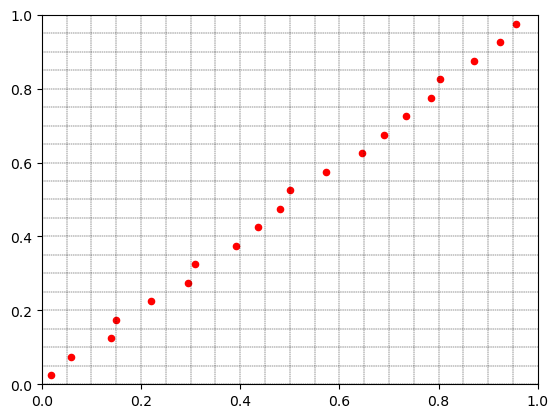
\includegraphics[width=\textwidth]{src/imgs/diagonal_poor_design.png}
        	\caption{A poor Latin Hypercube sampling in 2 dimension despite it fulfill the one-projection rule. This experiment shows how simple LHS can be insufficient to achieve a good simulation.}
        	\label{fig:diagonal_poor_design}
        }
    \end{subfigure}
    \hspace{0.05\textwidth}
    \begin{subfigure}[b]{0.45\textwidth}
        \centering
        \vtop{
        	\vspace{0pt}
        	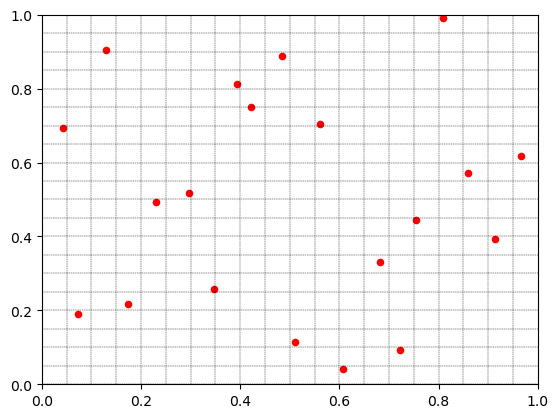
\includegraphics[width=\textwidth]{src/imgs/good_design.png}
        	\caption{This sampling has been generated using scipy LHSSampler utility class. The sample set bears random permutations of coordinates to lower the centered discrepancy. \ucite{scipy_lhs}}
        	\label{fig:good_design}
        }
    \end{subfigure}
	\caption{}
    \label{fig:latin_square}
\end{figure}

\subsubsection{Model-free and model-based simulation designs}
\label{subsubsec:model_free_model_based}
As the names may suggest, the latter implies the experimental design to involve some the peculiarities of the function to evaluate e.g. the shape that is expected, the initial or boundaries conditions, any well known critical region. Given that this approach is knowledge-driven, "What do we already know about?", can knock down pretty much the computational time required for the whole experiment with eventually high accuracy, but it can be equally easy that results may be deformed, based on assumptions that may prove wrong later, or make hard any further effort from other scientists to retake the experiment and confirm the results if the assumptions are not completely clear.
On the other hand, the model-free is the formal way to depict a fully independent sampling of the parameter space from the experiment which it has been designed for. Because of not many criteria have been left, all of the properties in this class are based on inter-element relationships, which convey that for each of them has a heuristic meant to quantify how much each sample is well-placed among the others. The shorthand for such a class of criteria is \textit{space-filling properties}.

Beside the many interesting considerations and suggestions that the model-based class of criteria has to offer to mathematicians, the space-filling properties has highly excited the experimenter community through the decades, producing creative and curious features that the samples could experience among each others. A very short list of the most representative ones is shown in \mtabref{tab:remarkable_criterions}. The most simple one is the [L2? phi di P?] criterion where the assumed metric is the Euler distance between each point in the hyperspace. The non-trivial issue comes along with the computational effort necessary to run through the search tree generated by the maximin (or minimax?) algorithm.

By the way, the characteristic non-collapsing property of the LHS itself is actually a space-filling property. It ensures that, for example, the average distance between the consecutive projections of a group of 3 samples on the same axis is at least 1/2 distance units and at most 3/2 d.u.

\begin{table}[h]
    \centering
    \begin{tabularx}{\textwidth}{X X X X} 
        \textbf{Authors} & \textbf{Year} & \textbf{Algorithm} & \textbf{Criteria} \\
        \hline
        \text{Audze and Eglajs} & 1977 & \text{Coordinates exchange} & \text{Potential energy} \\
    \end{tabularx}
    \caption{ Riempio la tabella piano piano che leggo i paper. Ho visto che molte ricerche su LHS usano dare una cronologia sull'utilizzo dei criteri utilizzati throught history}
	\label{tab:remarkable_criterions}
\end{table}

\section{Expansion of a Latin Hypercube Sampling}
\label{sec:lhs_expansion}

Given the problem outlined, it's necessary an heuristic which express how much the expanded issue is far away from a perfect expansion, given the starting state and the expansion magnitude desired. The \meqref{eq:grade} metric is not sufficient to achieve this, then it has been proposed the variant \meqref{eq:expanded_grade}. 
The "expanded grade" has been designed to reduce the sample set $S$ of $N$ elements to an percentage index when- here it differs from the previous definition of grade - the sample set is compared against a $P$-dimensional hypercube sectioned for an hypothetical LHS set of $N + M$ samples. Here it follows:
\begin{equation}
\label{eq:expanded_grade}
gr(S, M) := \frac{\sum^P_{j=1}\sum^{N + M}_{q=1} min(\sum^N_{i=1}\indfunc{[\frac{q-1}{N + M}, \frac{q}{N + M})}(S_{ij}), 1)}{P \cdot (N + M)}
\end{equation}


\section{APPENDIX}
\subsection{Indicator function}
\label{appendix:indicator_function}
The indicator function $\indfunc{}$ of a set \textbf{A} indicates whether the input belongs  to $A$ or not, specifically:
\begin{equation}
\label{eq:indicator_function}
\indfunc{A}(x) := 
\begin{cases}
1 \qquad \text{\textit{if x $\in$ A}}\\
0 \qquad \text{\textit{if x $\not\in$ A}}
 \end{cases}
\end{equation}
As in the matter of sectioning a space into continuous intervals in the shape of [a, b), it is useful to redefine the indicator function as an operation that occurs with the boundaries of $A$ using the Heaviside step function which does not involve set operators but only logical ones. It's important to remark that it doesn't matter what happens precisely on the boundaries. 
The Heaviside function is defined:
\begin{equation}
\label{eq:heaviside}
H(x) := 
\begin{cases}
1 \qquad \text{\textit{if x $\geq$ 0}}\\
0 \qquad \text{\textit{if x $<$ 0}}
\end{cases}
\end{equation}
So the indicator function can be also produced:
\begin{equation}
\label{eq:indicator_function_with_h}
\indfunc{[a,b)}(x) = H(x - a) \cdot H(b - x)
\end{equation}


\section*{DRAFTBOX}
Let's introduce the Latin Hypercube Sampling, a popular experimental sampling method, model-free....
In this paper we'll consider and discuss the scipy's LHS implementation for python $\geq$ v3 as it does implement the expected non-collapsing property and an optimize sequential space-filling design based on the Minimax rule [6] (?)

In this paper, authors have used different notable sampling methods for comparison purposes, here follows each of them along with a brief not of they prominent characteristics: \\
• Sobol' sequence as low-discrepancy sequence, when the percentage of a sequence's points that fall into an arbitrary set $Z$ is nearly proportionate to the measure of $Z$, the sequence so-called low-discrepancy;\\
• ...
\\
\\

- each sample in a $P$-dimensional hypercube identifies $P$ sub-hyperplanes (in $(P-1)$ dimensions) that pass through it and are parallel to one of the axes

- Talk about problems with space-filling, search trees ecc.

- why Granularity [1] ? Discrepancy

- Why has this paper been proposed ? The Least Computational Time Problem

- PLHS [2] ? no, I suppose 

- LHS and the problem of the so-called "expansion"

- In this paper the authors propose the implementation of the expansion algorithm for the LHS that can maximize space-filling properties and the projective property.

+ [remember to say that we are generating the sample sets using python scipy lhs implmenetation)

\printbibliography
\end{document}